\section{Software design description: pyProCT}



pyProCT is a clustering analysis software. As we stated earlier, correct usage of clustering analysis methods is not easy: right algorithm selection, better parameters estimation or appropriate result analysis are just some of the problems that CA tools user faces. However, we also showed that CA is present in a lot of different subjects and is used, or would be useful, to people with  limited knowledge both on algorithmic methods and statistics. On the other way around we also find that CA specialists may not be able to correctly assess the results of a clustering due to the nature of the data itself.

This clustering tool aims to reduce this gap by using five different algorithms and allowing the user to define a clustering goal or hypothesis. With this and some more options, most related to the parameter estimation of each method, it tries to find the best algorithm and it's parameters for the inputted data. This way, through a more "semantic" approach users can "guide" pyProCT without forcing them to deeply understand the pros and cons each method w.r.t to an specific kind of data.

To schedule the execution of the algorithms uses \hyperref[sec:docs]{\textbf{pyScheduler} controller}. It features three modes: sequential, parallel, using python's multiprocessing module, and parallel using MPI. The refactor will add fourth mode to run the tool with pyCOMPSs. It is important to note that the modifications will be limited to pyProCT, so COMPSs will act as a substitute of the current controller, not as a new scheduling method inside pyScheduler.



\subsection {Algorithms}

pyProCT uses the following five algorithms to find the best clustering. It also has an extra one which clusters the data randomly. This one is used for comparative purposes so it won't have more consideration that the utility it provides for other's behaviour analysis.

\begin{enumerate}

\item{K-medoids}
\item{Hierarchical}
\item{DBSCAN}
\item{GROMOS}
\item{Spectral}

\end{enumerate}

For more information about the actual implementation and parameter estimation of pyProCT check dropbox documentation on \ref{sec:docs} Documentation section.

\subsection{Execution Flow}
\label{sec:execution_flow}

The execution flow of pyProCT can be subdivided into four main sections linked to the JSON script structure:

\begin{description}
\item [Global,] \hfill \\ initialization of the software by reading parameters and options, parsing the JSON script, setting up the workspace and create the scheduler to be used.
\item [Data,] \hfill \\ construction of the distance matrix to be used. It offers three options: load, distance and rmsd.
\item [Clustering,] \hfill \\ calculation and evaluation of the clusterings.
\item [Postprocess,] \hfill \\ processing of the results to offer useful information about the clustering found.
\end{description}

On the next sections each part is going to be described, both it's execution flow and the json parameters associated with it.

\subsubsection{Global}

The global section is the responsible of initializing everything for the execution. This part is located on the main.py file and ends up calling the corresponding driver with the correct parameters. This is the main.py structure:

\begin{figure}[h]
\centering
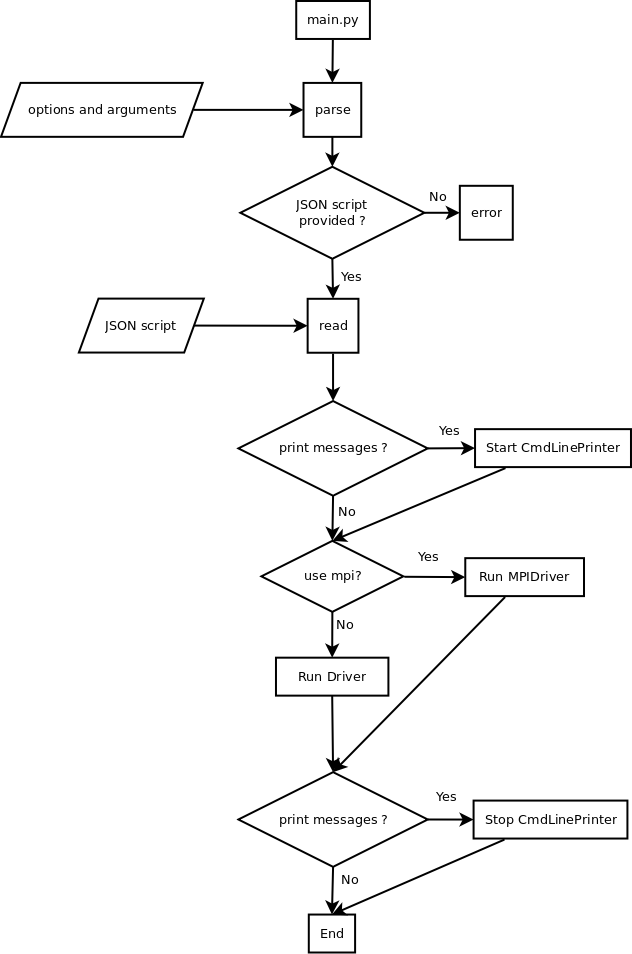
\includegraphics[height=0.5\paperheight]{img/global.png}
\caption{Global Section Execution Flow}
\vspace{1cm}
\end{figure}


This main file creates and initializes the Driver class which is the one orchestrating all the execution. Then the Driver class creates the workspace handler and saves the parameters before starting the Data, Clustering and Postprocess sections. The following figure shows encased in red the part corresponding to the global section inside the Driver. The next sections will expand the boxes Data, Clustering and Postprocess.

\begin{landscape}
\begin{figure}
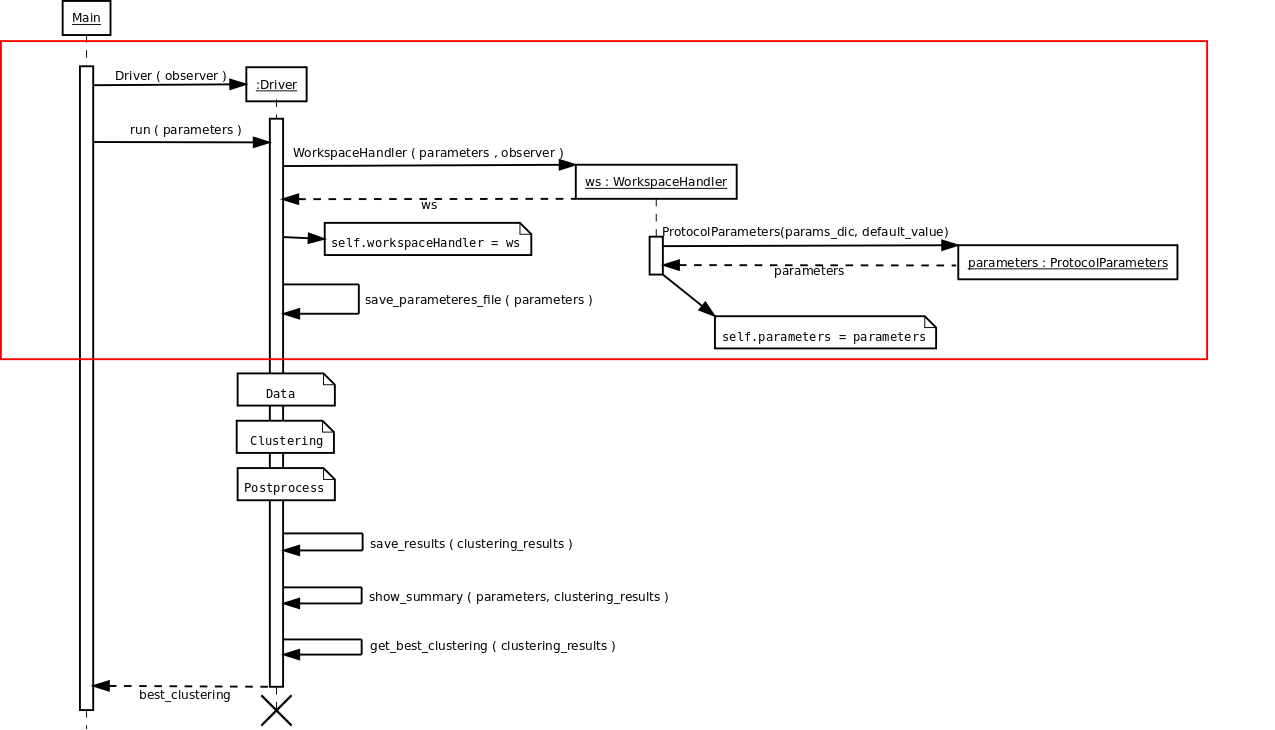
\includegraphics[width=25cm]{img/global_sequence_driver.jpg}
\caption{Global Section Execution Flow}
\end{figure}
\end{landscape}



The global section parameters that can be specified on the json file are divided into two groups: Control and Workspace. 

\begin{itemize}
\item \textbf{Control}
\begin{description}
\item [Scheduler type,] defines the kind of scheduler to use (serial, parallel, MPI or, after the refactor, pyCOMPSs)
\item [Number of processes,] if the parallel scheduler type is selected this option defines the number of processes to be used.
\end{description}
\item \textbf{Workspace}
\begin{description}
\item [Base,] is mandatory and defines the base workspace path.
\item [Tmp,] defines the folder to store temporal files.
\item [Matrix,] defines the folder to store the distance matrix (if applicable).
\item [Clusterings,] defines where cluster-related files are going to be stored, however the clusterings are stored as part of the results file.
\item [Results,] defines where the results file should be stored.
\item [Parameters:] \hfill
\begin{description}
\item [Overwrite,] if true, existing folders will be removed before execution.
\item [Clear after execution,] defines the folders to be removed after execution.
\end{description}
\end{description}
\end{itemize}


\subsubsection{Data}

This section defines how the distance matrix should be build. Essentially it runs the \textit{DataDriver}'s method \textit{run()} with the \textit{WorkspaceHandler} initialized on the global section and the retrieved parameters. This data driver initializes and returns to the main driver the \textit{DataHandler} and \textit{MatrixHandler} to be used later. The first one is directly instantiated with the corresponding parameters. The second one, on the other hand, first loads the matrix calculator defined on matrix's method of the json control file. With this calculator, the data handler and the parameters, it computes and returns the desired matrix handler. 

The following figure shows a simplified sequence diagram of this process:

\begin{landscape}
\begin{figure}
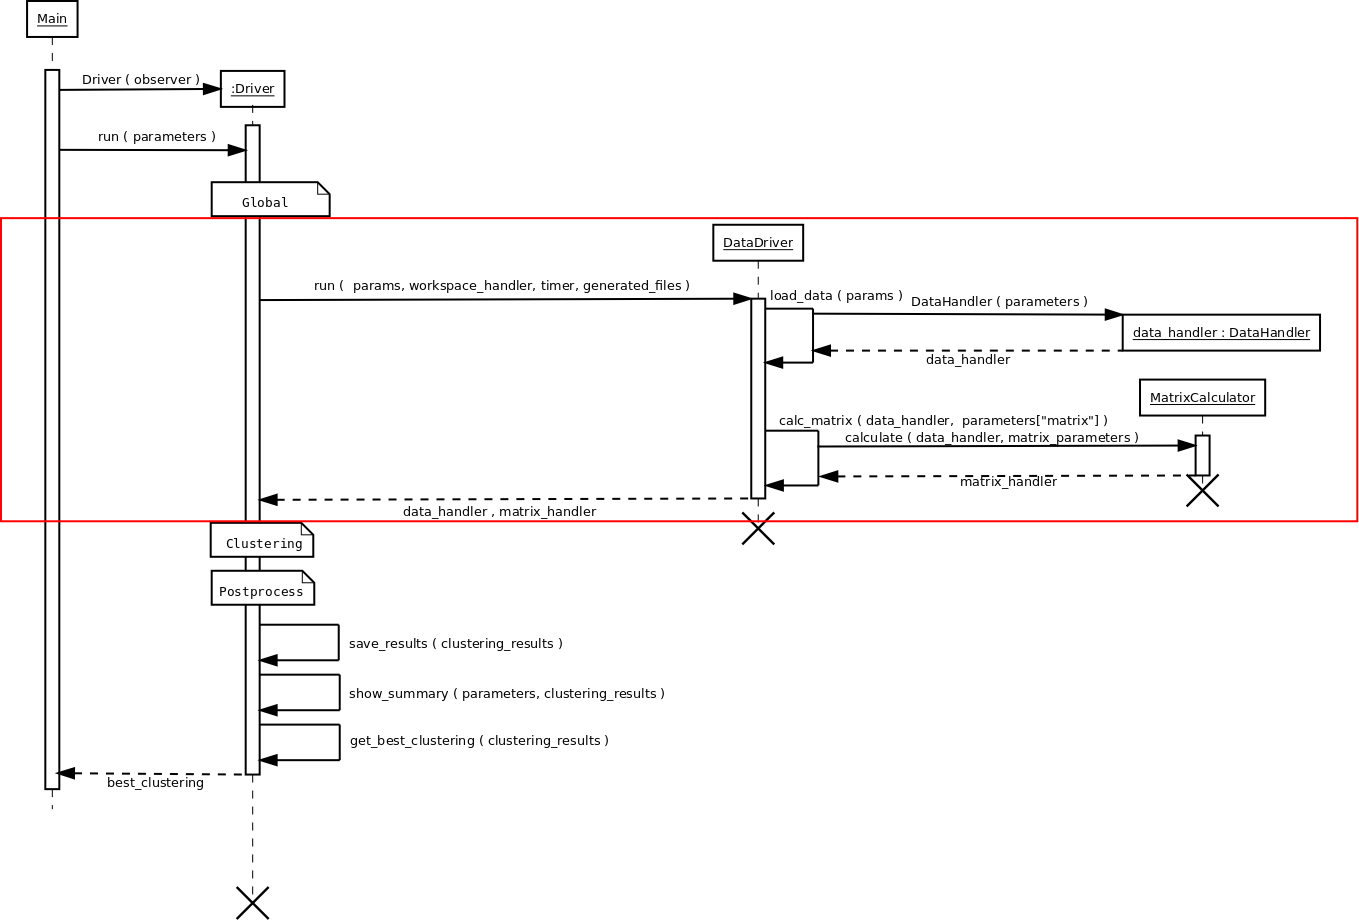
\includegraphics[width=24cm]{img/data_sequence_driver.png}
\caption{Data Section Execution Flow}
\end{figure}
\end{landscape}



The data section parameters specify the type and origin of the data, the method used to calculate the distance matrix and some more matrix-related parameters:


\begin{description}
\item [Type, ] sets the kind of data loader to use for the dataset.
\item [Files,] defines the location of the input files.
\item [Matrix] \hfil
\begin{description}
\item [Method,] selects the method used to calculate the distance matrix.
\item [Parameters,] allows to customize some parameters used to by the distance matrix calculator like:
\begin{description}
\item [Calculator Type,] must be one of the local pyRMSD installation available ones.
\item [Fit Selection,] for distance or rmsd methods.
\item [Body Selection,] for distance method.
\item [Calculate Selection,] for rmsd method.
\item [Path,] in case we are loading the matrix.
\end{description}
\item [Image,] setting this section will result in rendering a visual representation of the matrix.
\begin{description}
\item [Filename,] desired path of the rendered image.
\item [Dimension,] sets the leading dimension of the matrix image [default:1000px]
\end{description}
\item [Filename,] name of the file where the distance matrix will be saved (if applicable) inside the folder defined on workspace::matrix section. 
\end{description}
\end{description}


\subsubsection{Clustering}

This section is the one performing the actual clustering exploration and evaluation of the results. 

As \hyperref[fig:clustering_section]{Figure \ref{fig:clustering_section}} shows, the driver calls it's \textit{clustering\_section()} function which checks wether it needs to perform the exploration or load an existing clustering. 

If the method selected is "load" then the function \textit{from\_dic(...)} turns the data into a Clustering instance. 

If "generate" is the selected method then it calls \textit{perform\_clustering\_exploration(...)} which initializes and runs the \textit{ClusteringProtocol} class. This one, in turn, runs and initializes the classes  \textit{ClusteringExplorer}, \textit{ClusteringFilter}, \textit{AnalysisRunner} and the \textit{BestClusteringSelector}.

This clustering explorer deals with the actual exploration pipeline. It generates diverse parameter structures for each defined CA algorithm and adds them to the scheduler tasks queue, runs the scheduler and returns the resulting clustering\_info structures. 

The clustering filter tries to reduce the size of the clustering. To achieve this it eliminates the clusters whose parameters are outside the defined ranges on the evaluation section, removes the not selected clusters and checks that there are no repeated clusterings amongst the selected ones.

The analysis' runner is the one handling the evaluation of the selected clusterings. Similarly to \textit{ClusteringProtocol}, it creates an scheduler instance, queues the parametrization of each clustering analysis into it and runs it. Finally, it attaches the results to the clustering structure evaluated.

The BestClusteringSelector normalizes the calculated evaluations, scores each evaluation with the defined criteria and finally returns the id with higher score and the score itself.

Finally the ClusteringProtocol returns the clustering results containing:  \textit{best\_clustering\_id}, \textit{selected\_clusterings}, \textit{not\_selected\_clusterings} and \textit{all\_scores}. This results are then returned to the driver for the postprocessing section.

\begin{landscape}
\begin{figure}
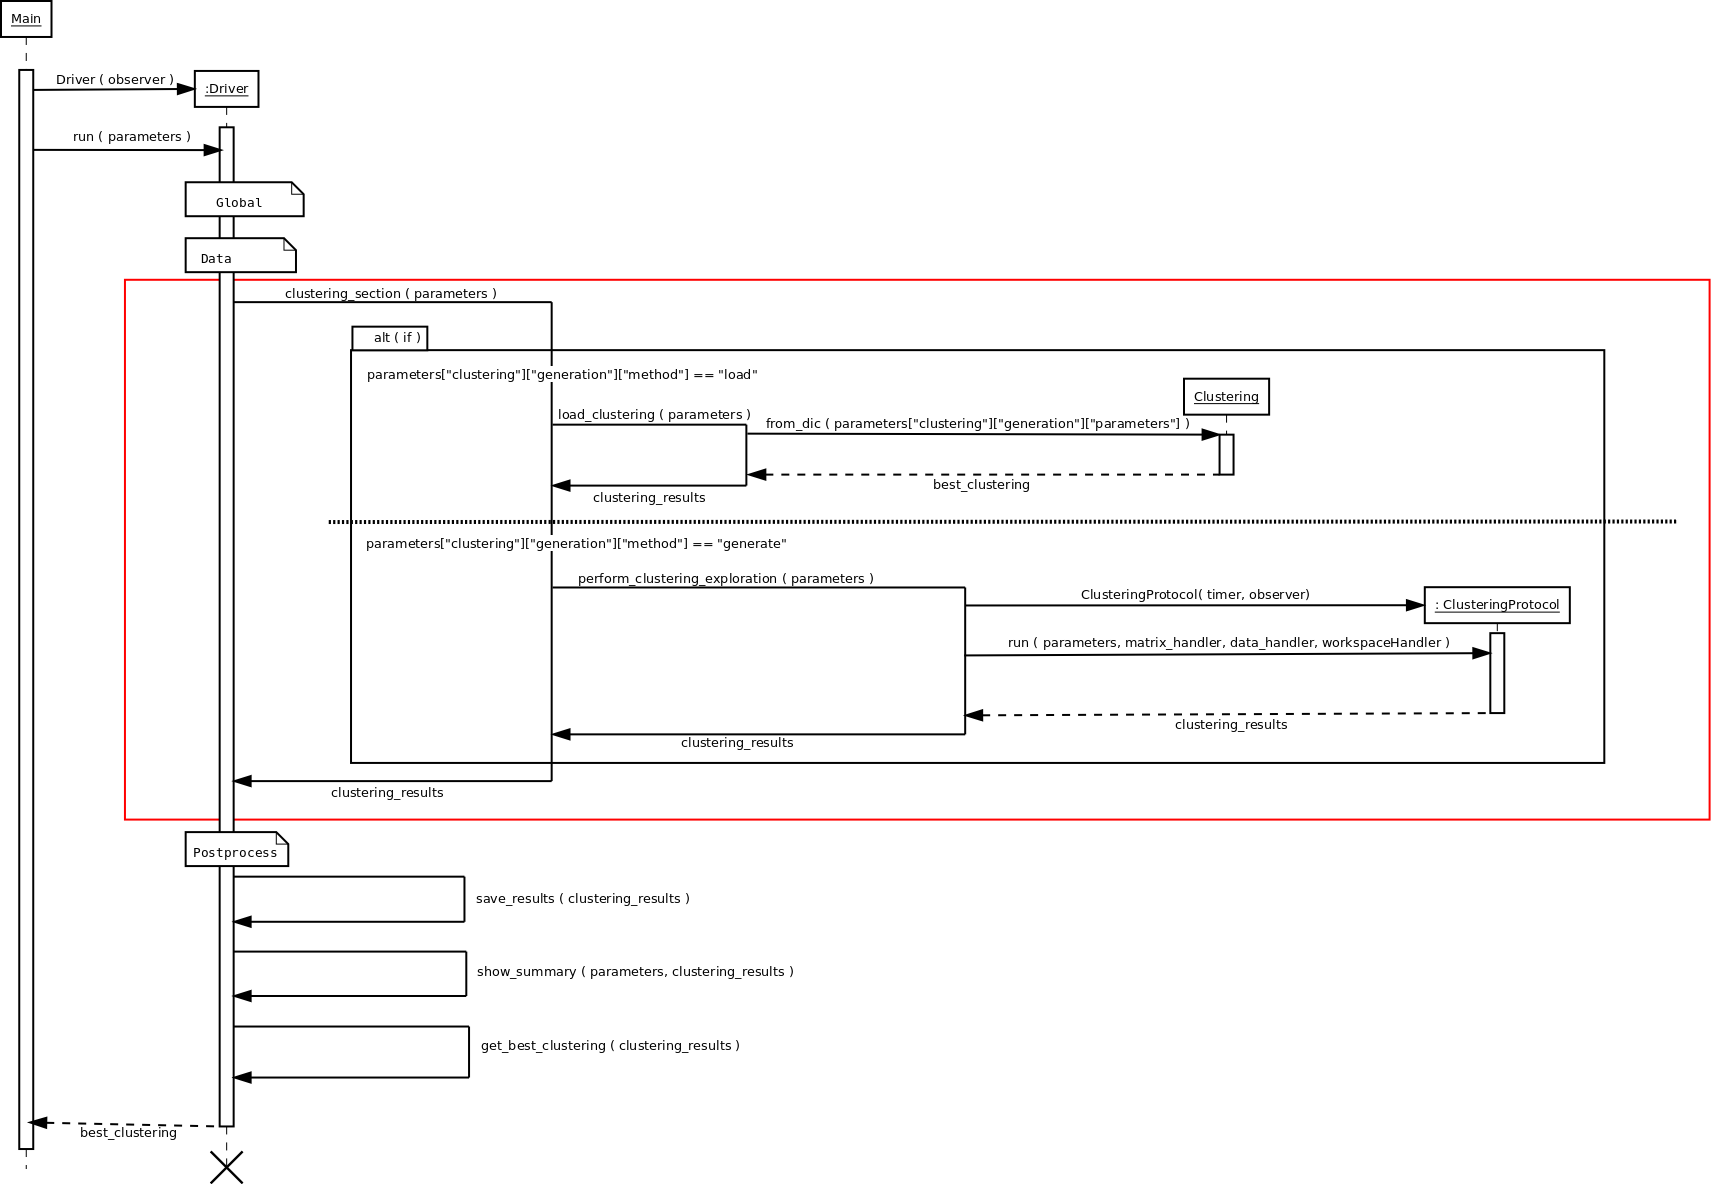
\includegraphics[width=24cm]{img/clustering_sequence_driver.png}
\caption{Clustering Section Execution Flow}
\label{fig:clustering_section}
\end{figure}
\end{landscape}



The clustering section parameters that can be specified on the json file define if the clustering should be generated or loaded, which algorithms and parameters to use and, finally, the evaluation section which is where the user should define his goal or hypothesis.

\begin{description}
\item [Generation] \hfil
\begin{description}
\item [Method,] selects wether we want to load or calculate the best clustering info. If it's loaded it will use the json dictionary defined on clustering::generation::clusters.
\item [Clusters,] clustering data if the method is "load". Each cluster object must define: id, prototype and elements.
\end{description}
\item [Algorithms,] \hfil \\for each desired algorithm to use of the six available (dbscan, gromos, hierarchical, kmedoids, random and spectral) defines it's parameters. All algorithms share the 'max', defining the maximim number of parametrizations for the algorithm, and the 'parameters' properties.
\begin{description}
\item [Kmedoids, ] \hfil 
\begin{description}
\item [Seeding type,] defines if the initial seeds should be randomly placed or at equidistant points.
\item [Tries,] if the initial seeds are to be randomly placed, this defines the number of repetitions done with different seeds (default: 10).
\end{description} 
\end{description}
\begin{description}
\item [Spectral, ] \hfil 
\begin{description}
\item [Sigma,] defines the sigma parameter for the spectral clustering. If not set, the default is to calculate local sigmas.
\end{description} 
\end{description}
\item [Evaluation] \hfil
\begin{description}
\item [Minimum clusters,] minimum number of clusters each clustering must contain to be evaluated.
\item [Maximum clusters,] maximum number of clusters a clustering must contain to be evaluated.
\item [Minimum cluster size,] any cluster smaller than this threshold will be considered noise (thus increasing the clustering noise).
\item [Minimum noise,] clusterings with higher noise than this threshold won't be evaluated.
\item [Query types,] list of details to be reported about the clustering found.
\item [Evaluation criteria,] list of criteria objects, each criteria containing one or more evaluation objects.
\begin{description}
\item [Evaluation object,] defines the sigma parameter for the spectral clustering. If not set, the default is to calculate local sigmas.
\begin{description}
\item [Name,] defining the quality function.
\item [Action,] defines wether the function should be maximized (">") or minimized ("<"). 
\item [Weight,] defines the relative weight of this quality function (not mandatory that they add up to 1).
\end{description}
\end{description} 
\end{description}
\end{description}



\subsubsection{Postprocess}

The postprocessing section's allows users to extract useful information about the clustering. This section is the only optional one amongst the four described. 

The Driver first gets the best clustering, which is the only remaining information needed to call the PostprocessingDriver class. The run method of this class loads all the available action classes and, for each one defined on the postprocessing section of the json file, runs it with the clustering information provided. The extracted information needs to be visualized with pyProCT GUI in some cases and saved into pdb files on the others (refer to \hyperref[subsec:postprocess:params]{Postprocessing Parameters} for more info)




\begin{landscape}
\begin{figure}
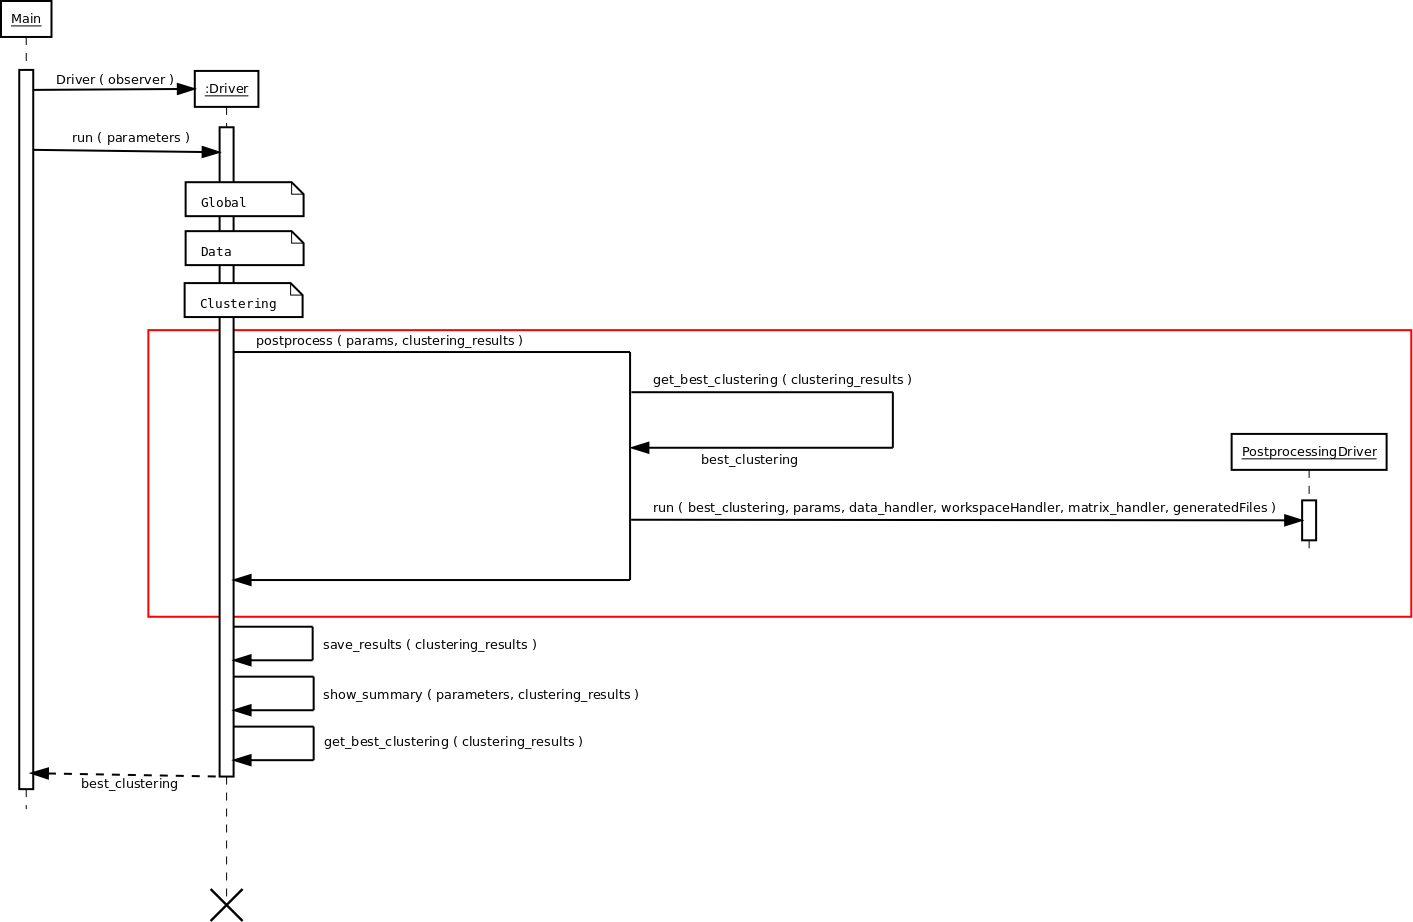
\includegraphics[width=24cm]{img/postprocess_sequence_driver.png}
\caption{Postprocess Section Execution Flow}
\end{figure}
\end{landscape}


\label{subsec:postprocess:params}
These are the possible postprocessing actions to be performed:


\begin{description}
\item [Rmsf,] pyProCT will generate the global and per-cluster
rmsf data to be visualized with the GUI.
\item [Centers and trace,] pyProCT will generate the data of all geometrical centers of the calculation selection of the system (to be visualized with the GUI)
\item [Representatives,] pyProCT will save the data of the medoid of each cluster on the best clustering in a pdb file.
\begin{description}
\item [Keep remarks,] if true, stored models will be saved with the their original remarks header (default: false).
\item [Keep frame number,] if set to true, the model number of any stored conformation will match the original pdb one (default: false).
\end{description}
\item [Pdb clusters,] pyProCT will save each cluster information in a pdb file.
\begin{description}
\item [Keep remarks,] if true, stored models will be saved with the their original remarks header (default: false).
\item [Keep frame number,] if set to true, the model number of any stored conformation will be the original pdb one. Default: false.
\end{description}
\item [Compression,] this option will produce a compressed version of the input trajectories with less redundancy thanks to the resulting clustering.
\begin{description}
\item [File,] name of the output file withouth extension (default:compressed.pdb)
\item [Final number of frames,] number of frames the compressed file must have.
\item [Type,] sampling method for cluster elements (default: kmedoids).
\begin{description}
\item [Random,] randomly samples elements for each cluster.
\item [Kmedoids,] uses k-medoids to get samples of the clusters.
\end{description}
\end{description}
\item [Cluster stats,] this will generate a human readable file with the distance among cluster centers and their diameters.  
\begin{description}
\item [File,] name of the generated file, without extension, to be stored inside results folder (default: per\_cluster\_stats.csv).
\end{description}
\end{description}

